\subsection{Oscillators}
\label{sec:oscillators}

Circuit parasitics can lead to the degradation of the FET gate signals. One way to grasp this effect is to look at the parasitic feedback circuit that leads to ringing and oscillation of the switches. For the sake of simplicity, the case of a single MOSFET is examined throughout Section \ref{sec:oscillators}. \\

This section is mainly based on a Toshiba application note \cite{Toshiba_app_note}.

\subsubsection{Causes of oscillation}
\label{sec:causes_of_osc}

False switching happens when a ringing or oscillating gate signal repeatedly turns the MOSFET on and off. This could cause excess power losses and permanent damage of the FET.

The three major causes of oscillation and ringing are the following: \\

\begin{itemize}
    \item An oscillation circuit is formed of the parasitic components and the feedback gain of the FET.
    \item A drain-source surge voltage during turn-off could reach the gate via feedback through the gate-drain capacitance $C_{GD}$.
    \item If the turn-off di/dt induces high enough voltage in the source stray inductances, the gate-source loop could go into LCR resonance. Stray inductance is a major contributor to potential ringing.
\end{itemize}

\subsubsection{Oscillation networks}
\label{sec:osc_network}

Oscillation happens when a circuit experiences voltage and current vibration without excitation from an external vibration source. Since all real-world circuits have resistance, oscillations dampen over time unless energy is fed into the network. In order for oscillation to occur, the feedback signal must match the phase and frequency of the input signal and have high enough amplitude to compensate for losses.

\subsubsection{Feedback circuit}
\label{sec:feedback_circuit}

The circuit in Figure \ref{fig:feedback_cl} shows the basic feedback network where

\begin{itemize}
    \item $v_i = $ input voltage
    \item $v_o = $ output voltage
    \item $A = $ loop gain
    \item $H = $ feedback factor
    \item $v_1 = $ input voltage applied to the amplifier
    \item $v_2 = $ feedback voltage
    \item $G_O = $ open-loop gain
    \item $G_C = $ overall, closed-loop gain
\end{itemize}

\begin{figure}[H]
	\centering
	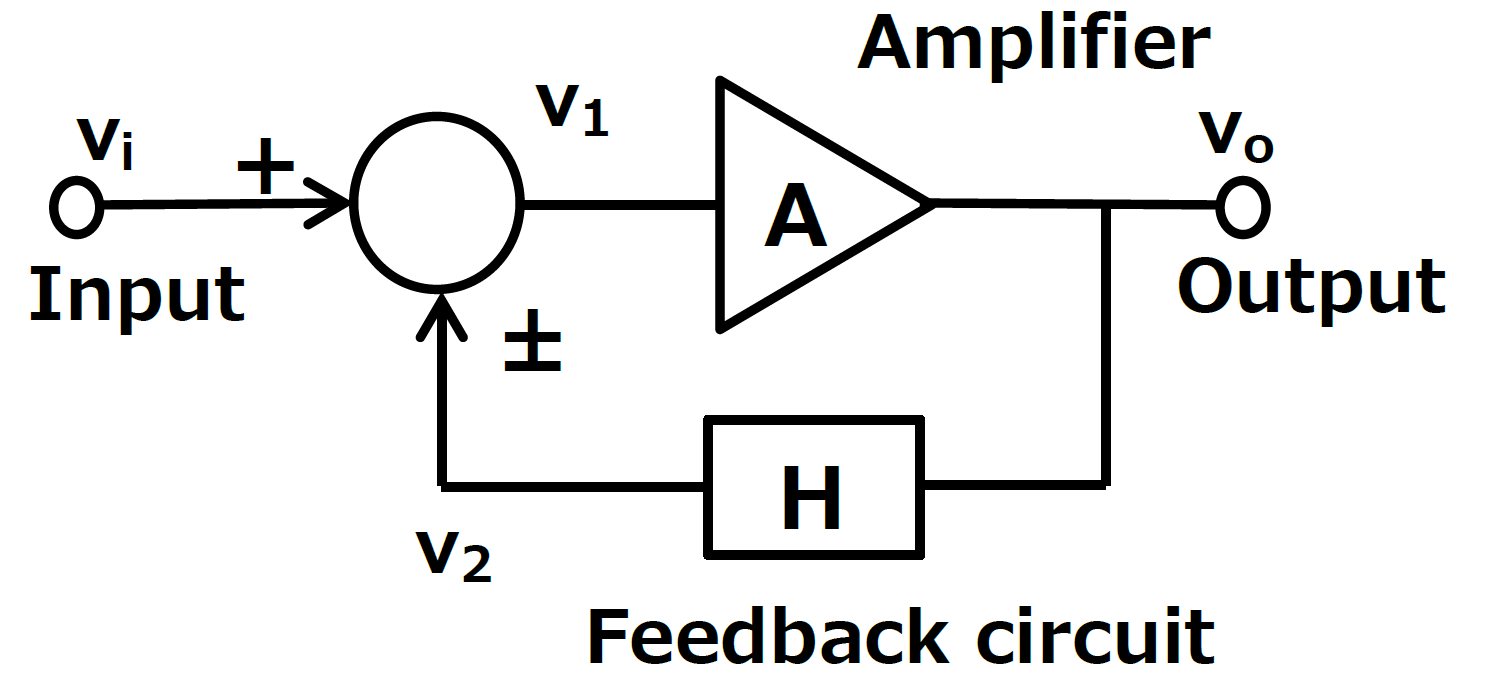
\includegraphics[width=0.4\textwidth]{pictures/theory/feedback_cl.png}
	\caption{Closed-loop feedback circuit}
	\label{fig:feedback_cl}
\end{figure}

To calculate the overall gain $G_C$, first, the open-loop transfer function should be specified:

\begin{equation}
    v_2 = AHv_1
\end{equation}

Dividing by $v_1$:

\begin{equation}
    G_O = \frac{v_2}{v1} = AH
\end{equation}

It can be seen that

\begin{equation}
    V_o = Av_1
\end{equation}

and

\begin{equation}
    V_1 = v_i + Hv_o
\end{equation}

combined yield

\begin{equation}
    v_o = A(v_i + Hv_o) = \frac{A}{1-AH}v_i
\end{equation}

From here, it is only one more step to get

\begin{equation}
    Gc = \frac{v_o}{v_i} = \frac{A}{1-AH}
    \label{eq:gc}
\end{equation}

\subsection{Circumstances for oscillation}
\label{sec:circumstances_for_osc}

If there is a positive feedback with $AH = 1$ from Equation \ref{eq:gc}; $G_c$ becomes infinite, prompting the network to oscillate. If we represent the $AH$ loop gain with a complex number of the form $a + jb$, oscillation occurs when $Re(AH) \geq 1$.

\subsubsection{MOSFET oscillation}
\label{sec:mosfet_osc}

If the parasitics are not keenly controlled, MOSFETs' high transconductance ($g_m$) and parasitic capacitances complemented by stray inductances make them susceptible to oscillation. $g_m$ is low when the MOSFET is in a steady state, so quick transient periods are of concern: when the load is shorted or switching occurs.

\subsubsection{MOSFET feedback loop}
\label{sec:mosfet_feedback_loop}

This section discusses the model for the single MOSFET feedback loop with ideal reactances seen in Figure \ref{fig:osc_model}. The resistance of the reactances is zero, current does not flow between the MOSFET and the reactances. Hence, Figure \ref{fig:osc_model2} is a good approximation.

\begin{figure}[H]
	\centering
	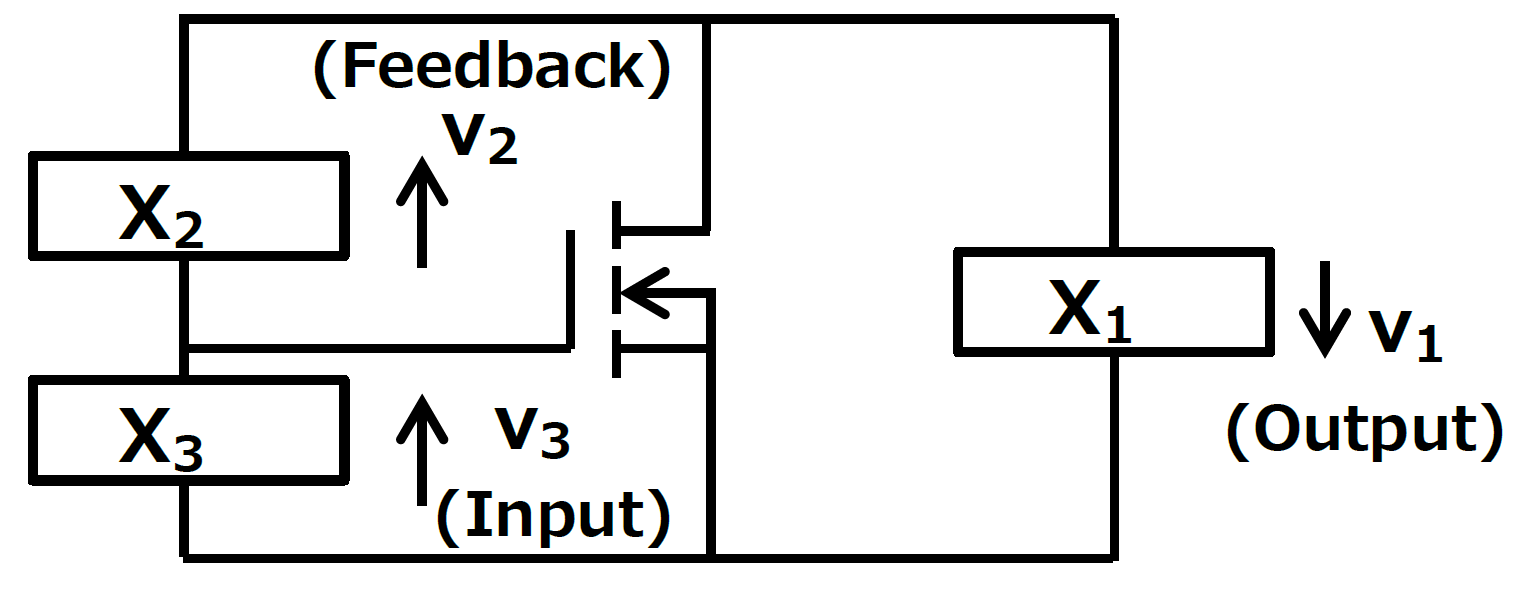
\includegraphics[width=0.4\textwidth]{pictures/theory/feedback_model.PNG}
	\caption{Circuit of an oscillation model}
	\label{fig:osc_model}
\end{figure}

\begin{figure}[H]
	\centering
	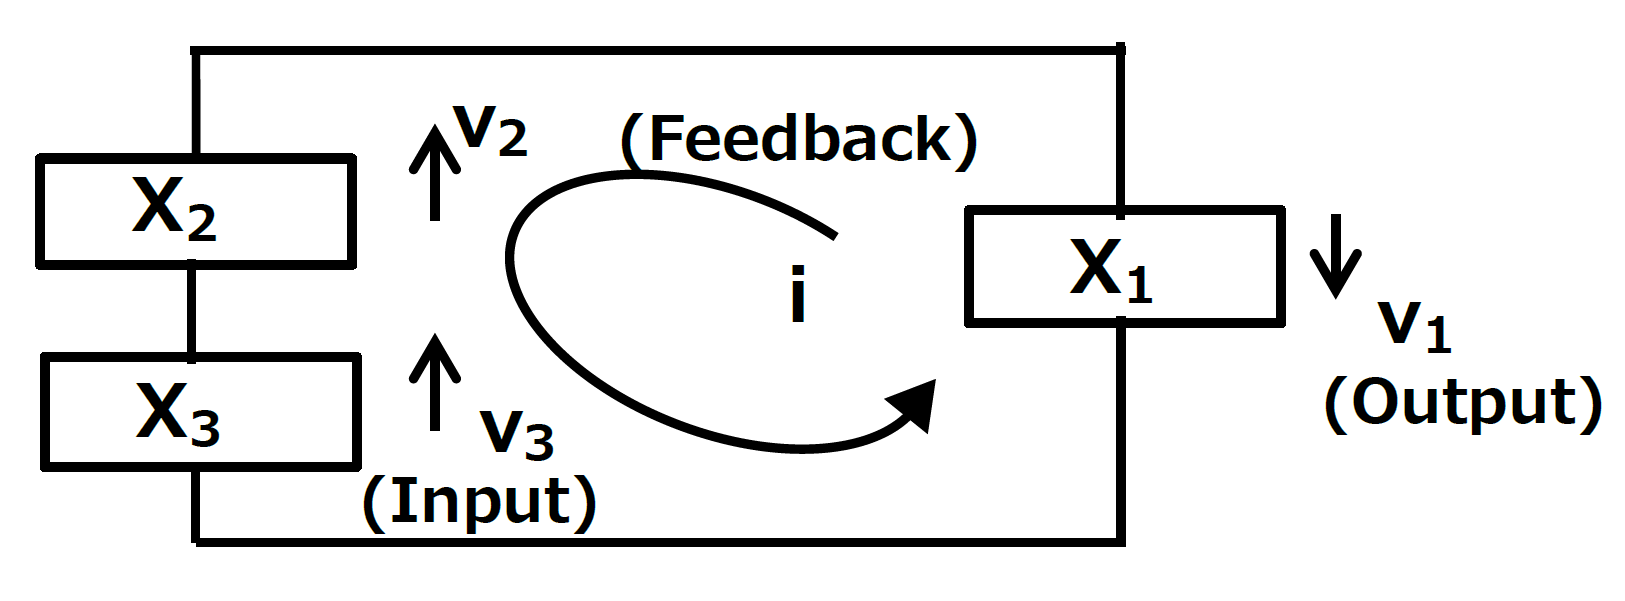
\includegraphics[width=0.4\textwidth]{pictures/theory/feedback_model_2.PNG}
	\caption{Current in the oscillation network}
	\label{fig:osc_model2}
\end{figure}

Kirchhoff's laws applied to Figure \ref{fig:osc_model2} yield

\begin{equation}
    v_1+v_2+v_3 = i(X_1+X_2+X_3) = 0
\end{equation}{}

and $i \neq 0 $ so

\begin{equation}
X_1+X2+X_3 = 0
\end{equation}

must be true. \\

The positive feedback loop can only occur when the input is in phase with the output. This happens when $X_1$ and $X_3$ are of the same property and $X_2$ is different. Circuits fulfilling the above requirements are Colpitts (Figure \ref{fig:colpitts_1}) and Hartley (Figure \ref{fig:hartley_1}) oscillators.

\begin{figure}[H]
	\centering
	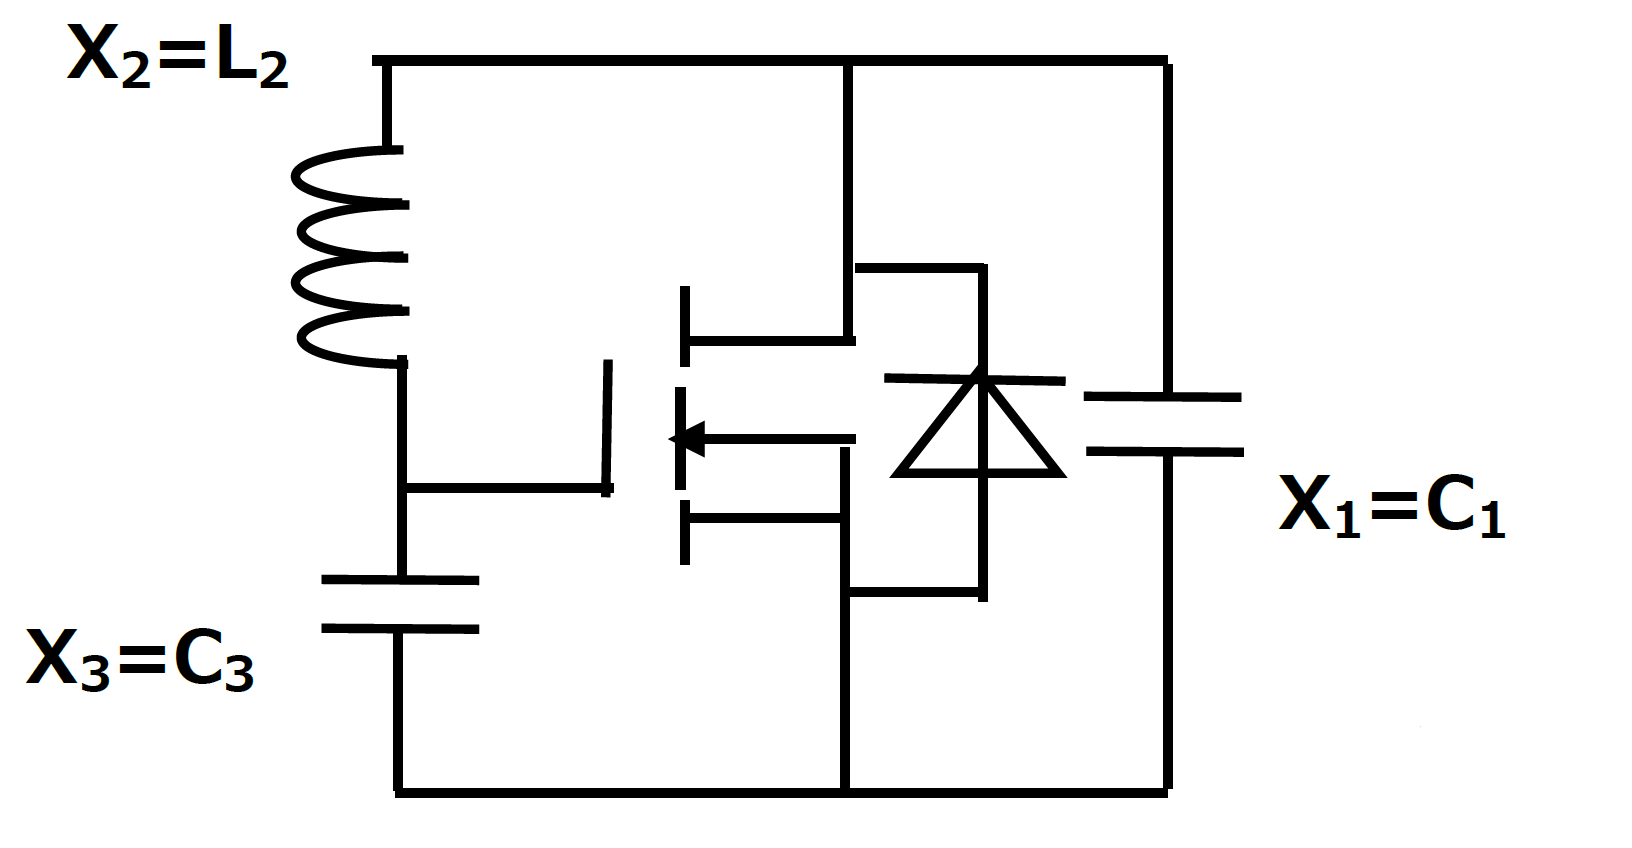
\includegraphics[width=0.4\textwidth]{pictures/theory/colpitts_1.PNG}
	\caption{Colpitts oscillator}
	\label{fig:colpitts_1}
\end{figure}

\begin{figure}[H]
	\centering
	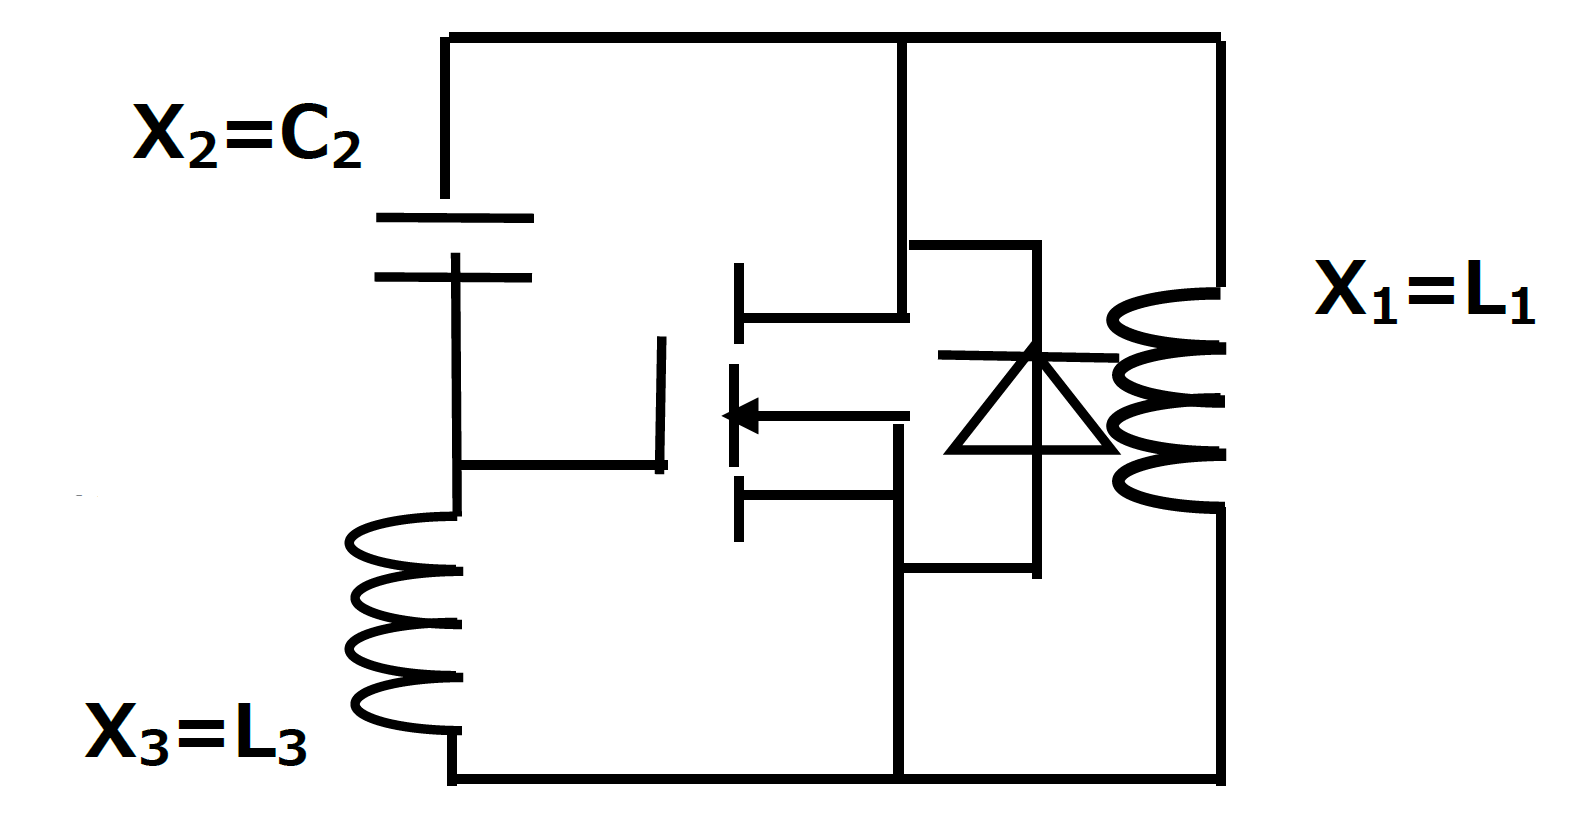
\includegraphics[width=0.4\textwidth]{pictures/theory/hartley_1.PNG}
	\caption{Hartley oscillator}
	\label{fig:hartley_1}
\end{figure}

\begin{figure}[H]
	\centering
	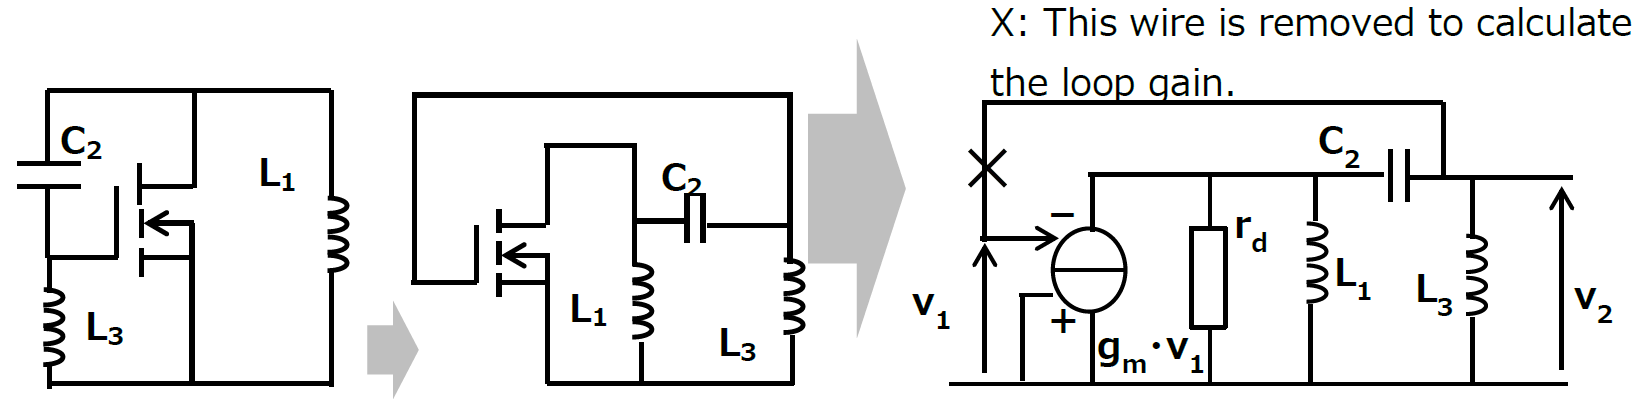
\includegraphics[width=\textwidth]{pictures/theory/hartley_2.PNG}
	\caption{Equivalent circuit of Hartley oscillator}
	\label{fig:hartley_2}
\end{figure}

Writing up the transfer function based on Figure \ref{fig:hartley_2} and performing further arithmetic actions yields the following:


\begin{equation}
    \omega = \frac{1}{\sqrt{(L_1 + L_3)C_2}}
    \label{eq:omega_hartley}
\end{equation}

\begin{equation}
    g_m \cdot r_D \geq \frac{L_1}{L_3}
    \label{eq:gain_hartley}
\end{equation}

Equation \ref{eq:omega_hartley} and \ref{eq:gain_hartley} gives the formula for calculating the oscillation frequency and the loop gain for a given set of parameters.

\subsection{Ringing}
\label{sec:ringing}

When switching off the MOSFET, drain di/dt and stray inductances can cause a $V_{DS}$ voltage surge that gets coupled to the gate. This ringing voltage can perturbate the gate signal so greatly that it repeatedly turns on and off, driving the MOSFET into oscillation. \\

The amplitude of the surge voltage depends on the value of the parasitic inductance and the changing rate of the drain current:

\begin{equation}
    V_{Surge} = L_{S2} \frac{di}{dt}
\end{equation}

\begin{figure}[H]
	\centering
	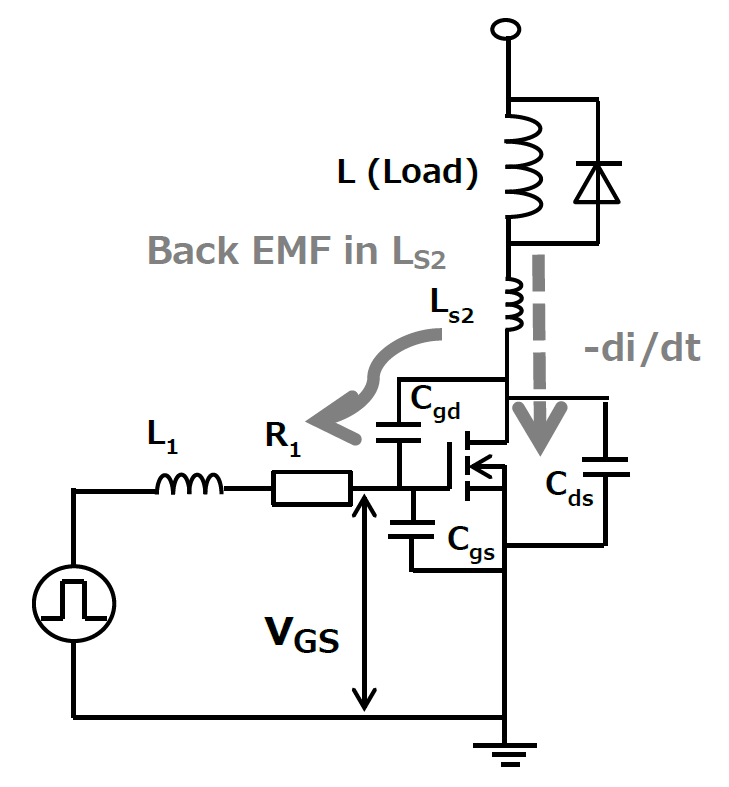
\includegraphics[width=0.4\textwidth]{pictures/theory/ringing_coupling.PNG}
	\caption{Ringing waveforms}
	\label{fig:ringing_coupling}
\end{figure}

The voltage gets coupled to the gate via $C_{gd}$, resulting in waveforms similar to those of in Figure \ref{fig:ringing_wf}

\begin{figure}[H]
	\centering
	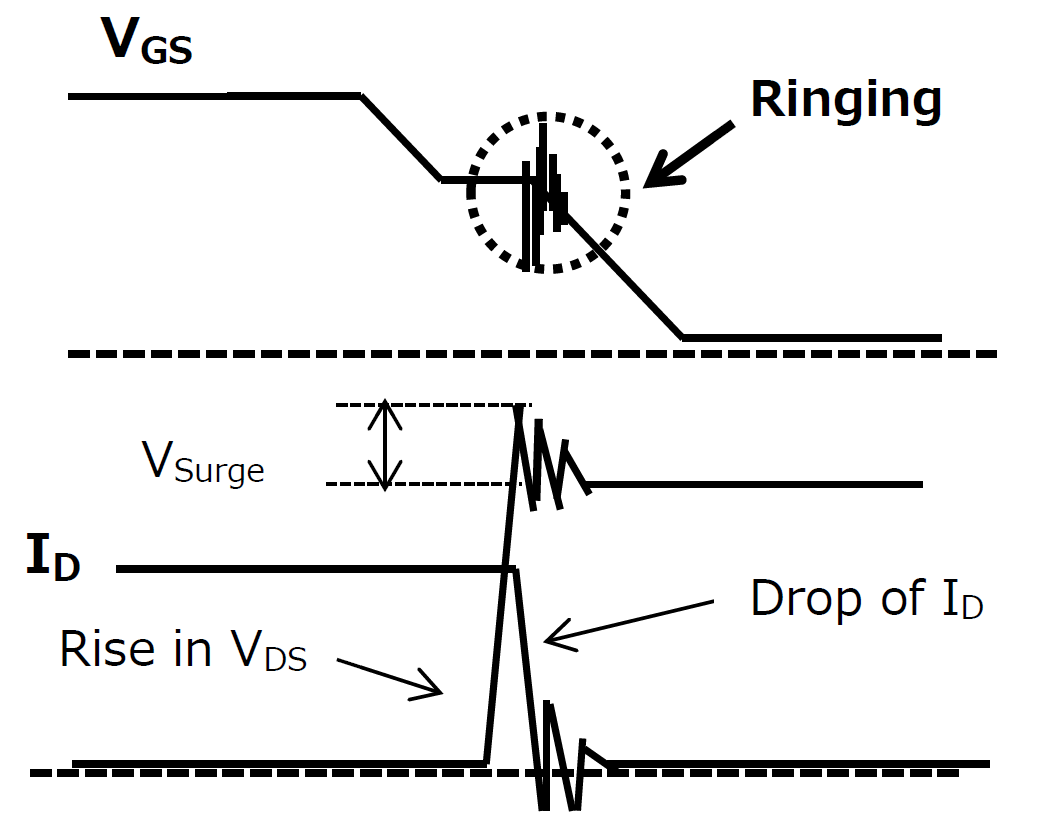
\includegraphics[width=0.4\textwidth]{pictures/theory/ringing_wf.PNG}
	\caption{Ringing waveforms}
	\label{fig:ringing_wf}
\end{figure}

High gate inductance and high driver turn-on currents associated with quick switching can also cause ringing. Dampening it by adding a resistor to the gate track brings additional losses. Furthermore slowing switching down increases the time slot when the MOSFET is subject to voltage and current at the same time, further increasing losses. Additional resistance may also prohibit operation at the desired frequency. Reducing parasitic inductances proves to be the desired action again.